\section{Information Theory Bounds \label{sec:information}}

We recall the idea of channel capacity with a simple example. Suppose that the latent variable $Y$ to be encoded is a symbol drawn from an alphabet of size $N.$ What is the minimum dimension $d$ such that each value of $Y$ can be represented by a vector $X \in \R^d$?

When the vector $X$ can be stored exactly, the answer to our question simply depends on the number of values it can take. If the coefficients of $X$ are $16$ bit floating point numbers, then each coefficient can store (nearly) $2^{16}$ distinct numbers, and overall we need only about $d_\text{min} \approx \frac 1 {16} \log_2 N$ dimensions.

However, we expect that activation vectors within real neural networks are subject to various kinds of interference. For example, an activation vector $X$ may need to represent the symbol $Y$ while also holding information on another latent quantity, or it may be subject to explicitly induced noise like dropout. Characterizing the ``capacity'' of a vector in the presence of interference is a basic problem in coding theory.

One common model is to consider that $X$ is subject to additive white Gaussian noise. More specifically, we let $Z \in \R^d$ be a vector of independent, centered Gaussians each of variance $P,$ and consider the problem of recovering $Y$ from $X + Z.$ The following is then a typical (but remarkable) result of information theory.

\begin{proposition} \label{prop:information}
    Let the random variable $Y \in [N]$ be uniformly distributed, and let $Z$ be white Gaussian noise of variance $P.$ Suppose there exist a pair of maps $F \colon [N] \to \R^d$ and $G \colon \R^d \to [N]$ so that
	$$
		G(F(Y) + Z) = Y
	$$
	with probability at least $(1 - p),$ and suppose the variance of each coordinate of $F(Y)$ is bounded by $1.$ Then
	$$
	d \geq 2 \frac{(1 - p) \ln N - \ln 2}{\ln \bigl( 1 + P^{-1} \bigr)}.
	$$
\end{proposition}

In particular, if we fix $P$ and let the number $N$ of symbols grow to infinity, this shows that the minimum dimension $d$ of a reliable code must grow logarithmically in $N.$ More specifically, we can say the following.

\begin{corollary} \label{prop:information-simple}
    Fix $P > 0,$ $\epsilon > 0,$ and suppose
    $$
    d \le \left(\frac 2 {\ln(1 + P^{-1})} - \epsilon\right) \ln N.
    $$
    Then, when the random variables $(Y, Z)$ and the maps $(F, G)$ are in the conditions of \Cref{prop:information}, the maximum value of $\Pp(G(F(Y) + Z) = Y)$ converges to $0$ for sufficiently large $N.$
\end{corollary}

Since $\ln(1 + P^{-1})^{-1} \approx P$ for large $P,$ this means that roughly $d \ge 2 P \ln N$ dimensions are needed to reliably code for $Y.$

Now, one very simple way to construct maps $F$ and $G$ is to choose the codewords $F(i)$ randomly from some distribution on the unit sphere in $\R^d$ and let $G(v)$ return the element $j$ so that $\langle v, F(j) \rangle$ is maximized. For brevity, we refer to $(F, G)$ This strategy can be motivated by the remarkable fact that random codebooks of size $\Omega(e^d)$ of $d$-dimensional codewords can have bounded interference, in the sense of the following result.

\begin{proposition} \label{prop:random-information}
    Let $(F, G)$ be constructed according to the random codebook strategy, let $\epsilon > 0,$ and let
    $$
    d \ge (2 + \epsilon) P \ln N.
    $$
    Then, when the random variable $(Y, Z)$ are in the conditions of \Cref{prop:information}, $\Pp(G(F(Y) + Z) = Y)$ converges to $1$ for large $N.$
\end{proposition}

Altogether, this shows that transmitting

\begin{figure}
	\begin{minipage}[c]{0.5\textwidth}
	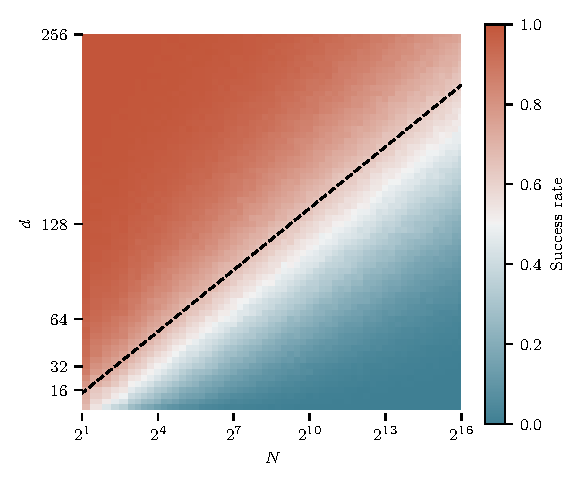
\includegraphics[width=\textwidth]{../figures/symbol_transmission}
	\end{minipage}%
	\begin{minipage}[c]{0.5\textwidth}
	\vspace{20pt}
	\caption{How many dimensions $d$ does the vector $X \in \R^d$ need to have for $X + Z$ to reliably code for an element $Y \in [N]$? This figure shows empirical success of the random codebook strategy when $Z$ is white noise with components of power $P.$}
	\label{fig:transmission}
	\end{minipage}
\end{figure}

Our discussion so far parallels many \cite{cover_elements_2006}. In the remainder of this work, we consider

It will also be useful to know the upper bound
$$
	H = \ln \binom N k \le k \ln (eN/k) = k \ln N - k \ln k + k
$$
on the entropy of a random $k$-element subset of $[N],$ which turns out to be a very good approximation when $k \ll N.$ For example, when $N = 2^{20}$ and $k = 2^8,$ the approximation
$$
	\ln \binom{2^{20}}{2^8} \approx 2^8 \ln(2^{20} e/2^8) = 128 (1 + 12 \ln 2)
$$
holds with a relative error of only about $0.3 \%.$ (See \Cref{appendix:binomial} for a discussion of this estimate.)
